\documentclass{beamer}
\usetheme{PaloAlto}
\usepackage{graphicx, color, hyperref}
\usepackage[utf8]{inputenc}
\usepackage[T1]{fontenc}
\usepackage{listings}

\title[Apresentação]{Ponteiros e árvores binárias}
\author[\textit{Kenji Yamane}]{Kenji Yamane}
\date{Abril de 2020}

\setlength{\parindent}{20 pt}

\begin{document}

\begin{frame}

\titlepage

%\begin{figure}
%	\includegraphics[width=30 pt]{c-symbol}
%	\hspace{20 pt}
%	\includegraphics[width=30 pt]{cpp-symbol}
%	\label{c and cpp}
%\end{figure}

\end{frame}

\begin{frame}

\frametitle{Tópicos da aula}

\tableofcontents

\end{frame}

\section{Ponteiros}
	
	\begin{frame}
	\frametitle{Alocação dinâmica}
		Para trabalhar com árvores binárias, precisa-se
		primeiramente aprofundar-se um pouco mais no assunto de
		ponteiros. Comentou-se sobre como ele pode ser usado para
		apontar para variáveis normais; por exemplo, se for necessário
		fazer um ponteiro p apontar para uma variável inteira x, basta
		fazer:
		\begin{block}{Código 1}
		\hspace{10 pt} int x = 5;\\
		\hspace{10 pt} int *p = \&x;
		\end{block}
		Pois o operador \& retorna o endereço da variável x. Agora,
		é possível também criar uma "variável", ou seja um espaço de
		memória somente a partir de ponteiros, porém ele deve ser
		criado e deletado manualmente, conforme mostra o código do
		próximo slide, utilizando comandos de C++.
	\end{frame}

	\begin{frame}[fragile]
	\frametitle{Código 2}
		\begin{lstlisting}
#include <iostream>

int main() {
    int *p = new int;
    *p = 5;
    delete p;

    return 0;
}
		\end{lstlisting}
	\end{frame}

	\begin{frame}
	\frametitle{Operador seta}
	Além disso, também se trabalhará com ponteiros de struct.
	Devem se lembrar das aulas de treinamento de C que se acessa
	o que se tem dentro de uma variável de struct através do ponto
	(.). Se for um ponteiro para struct, as variáveis de dentro da
	struct são acessadas com seta (->), como mostra o código
	abaixo.
	\end{frame}

	\begin{frame}[fragile]
	\frametitle{Código 3}
		\begin{lstlisting}
#include <iostream>

struct par {
    int first;
    int second;
}

int main() {
    par *p = new par;
    p->first = p->second = 1;
    printf("%d %d\n", p->first, p->second);
    delete p;

    return 0;
}
		\end{lstlisting}
	\end{frame}

	\section{Árvores binárias por struct}
	\begin{frame}
	\frametitle{O que é uma árvore binária}
		Agora pode-se iniciar os estudos de árvores binárias:
		compostas por um nó raiz, que aponta para dois filhos, um
		correspondente à uma "raiz" de uma sub-árvore esquerda, e um
		correspondente à uma "raiz" de uma sub-árvore direita. Cada
		nó pode ter no máximo dois filhos.

		\begin{figure}[H]
			\centering
			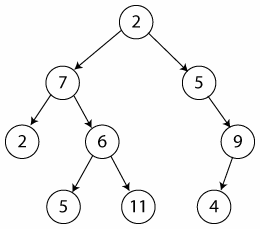
\includegraphics[width=4cm]{binary_tree.png}
		\end{figure}
	\end{frame}

	\begin{frame}
	\frametitle{Em C++}
		Já é possível imaginar, dos termos usados no último slide,
		como se construiria uma árvore binária em C++: uma struct
		que possui três membros: uma informação, um ponteiro
		apontando para o filho esquerdo, e um ponteiro apontando para
		o filho direito. Para construir por exemplo uma árvore simples
		que tem uma raiz com o valor 2 e filho esquerdo com valor 1 e
		filho direito com valor 7, utilizaria-se do código 5.
		\begin{block}{Código 4}
		\hspace{10 pt} struct tree \{\\
		\hspace{20 pt} int info;\\
		\hspace{20 pt} tree *left;\\
		\hspace{20 pt} tree *right;\\
		\hspace{10 pt} \}
		\end{block}
	\end{frame}

	\begin{frame}[fragile]
	\frametitle{Código 5}
		\begin{lstlisting}
int main() {
    tree *rightSon = new tree;
    tree *leftSon = new tree;
    tree *root = new tree;

    rightSon->info = 7;
    rightSon->left = rightSon->right = NULL;
    leftSon->info = 1;
    leftSon->left = leftSon->right = NULL;
    root->info = 2;
    root->right = rightSon;
    root->left = leftSon;

    return 0;
}
		\end{lstlisting}
	\end{frame}

	\begin{frame}
	\frametitle{Deletando a árvore}
		Perceba que não foi realizado o delete. Dado que foi criado
		com um ponteiro, o delete deve ser feito manualmente. Se ele
		não for, a memória continua sendo usada, o que se chama de
		memory leak. Admito que eu creio que a maioria dos juízes
		online não se importa com isso, mas é bom evitar e ajuda na
		didática da aula mostrar: como deletar uma árvore? Tem de ser
		uma ideia que funcione também para quando a árvore ficar bem
		complicada. Não se pode deletar a raiz antes de deletar os
		filhos senão se perde o acesso aos filhos. Isso se resolve
		recursivamente: caso se procure deletar uma árvore t, primeiro
		deleta-se a sub-árvore esquerda, depois a sub-árvore direita, e
		finalmente se deleta t. Não se deleta t se ele for NULL, que é o
		ponteiro que não aponta para nada, usado como ponto de
		parada nesse algoritmo.
	\end{frame}

	\begin{frame}[fragile]
	\frametitle{Código 6}
		\begin{lstlisting}
void delete_tree(tree *t) {
    if (t != NULL) {
        delete_tree(t->left);
        delete_tree(t->right);
        delete t;
    }
}
		\end{lstlisting}
	\end{frame}

	\begin{frame}
	\frametitle{Exploração de árvores}
		Serão expostas três formas de exploração de árvores aqui.
		Sabe-se que caso se queira explorar uma árvore t, é necessário
		explorar o nó t (usado para imprimir nesse caso), explorar a
		sub-árvore esquerda, e a sub-árvore direita. Há três formas
		possíveis de exploração(sub-árvore esquerda sempre antes da
		direita), a primeira sendo explorar o nó e depois os filhos,
		chamada de pré-ordem:
		\begin{block}{Código 7}
		\hspace{10 pt} void explore(tree *t) \{\\
		\hspace{20 pt} if (t != NULL) \{\\
		\hspace{30 pt} cout << t->info << endl;\\
		\hspace{30 pt} explore(t->left);\\
		\hspace{30 pt} explore(t->right);\\
		\hspace{20 pt} \}\\
		\hspace{10 pt} \}
		\end{block}
	\end{frame}

	\begin{frame}
	\frametitle{Exploração de árvores}
		O NULL é usado novamente como ponto de parada, e
		recursão é novamente usado. A outra forma se chama
		in-ordem, ou ordem simétrica. Nela, se explora primeiro a
		sub-árvore esquerda, depois a raiz, e então a sub-árvore direita.
		\begin{block}{Código 8}
		\hspace{10 pt} void explore(tree *t) \{\\
		\hspace{20 pt} if (t != NULL) \{\\
		\hspace{30 pt} explore(t->left);\\
		\hspace{30 pt} cout << t->info << endl;\\
		\hspace{30 pt} explore(t->right);\\
		\hspace{20 pt} \}\\
		\hspace{10 pt} \}
		\end{block}
	\end{frame}

	\begin{frame}
	\frametitle{Exploração de árvores}
		A terceira e última forma consiste em primeiro explorar os
		filhos e somente depois explorar a raiz, chamada pós-ordem.
		Novamente se utiliza recursão:
		\begin{block}{Código 9}
		\hspace{10 pt} void explore(tree *t) \{\\
		\hspace{20 pt} if (t != NULL) \{\\
		\hspace{30 pt} explore(t->left);\\
		\hspace{30 pt} explore(t->right);\\
		\hspace{30 pt} cout << t->info << endl;\\
		\hspace{20 pt} \}\\
		\hspace{10 pt} \}
		\end{block}
		Perceba que deletar uma árvore é simplesmente um
		percurso pós-ordem, que se aproveita do fato de que na
		pós-ordem, primeiro os filhos são visitados.
	\end{frame}

	\begin{frame}
	\frametitle{Exploração de árvores}
		Uma representação gráfica dos três tipos de percurso estão
		mostradas a seguir (a linha tracejada é a exploração e ela
		explora o nó no ponto vermelho). Veja que as figuras
		correspondem aos algoritmos recursivos.
		\begin{figure}[H]
			\centering
			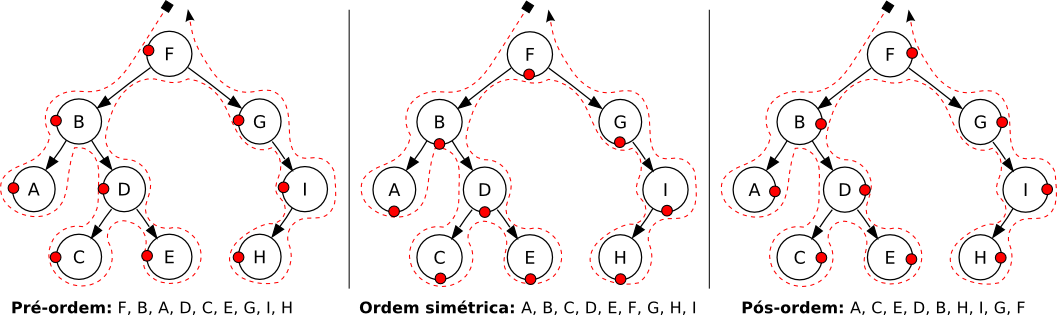
\includegraphics[width=10cm]{tree_exploration.png}
		\end{figure}
	\end{frame}

	\section{Árvores Binárias de Pesquisa}

	\begin{frame}
	\frametitle{O que são ABP's}
		Árvores Binárias de Pesquisa são árvores binárias especiais
		no sentido de que: todos os números que estão na sub-árvore
		esquerda de uma raiz são menores do que a raiz, e todos os
		números da sub-árvore direita da raiz são maiores que ela.
		Qualquer sequência de números pode gerar uma ABP, lendo
		número por número, e inserindo cada um na árvore. A forma de
		inserção leva em conta a característica da ABP e usa recursão
		também, como mostrado no próximo slide.
	\end{frame}

	\begin{frame}[fragile]
	\frametitle{Código 10}
		\begin{lstlisting}
tree* insert(tree *t, int value) {
    if (t == NULL) {
        t = new tree;
        t->info = value;
        t->left = t->right = NULL;
    } else if (value < t->info)
        t->left = insert(t->left, value);
    else
        t->right = insert(t->right, value);

    return t;
}
		\end{lstlisting}
	\end{frame}
	
	\begin{frame}
	\frametitle{Propriedades de ABP's}
		Os benefícios principais das ABP's são dois: o percurso
		infixo deles gera a sequência ordenada (se a sub-árvore esquerda
		é impressa antes da raiz e a direita depois, a raiz está na
		posição certa, e isso é válido recursivamente para qualquer nó).
		O outro, o mais importante, é que a busca nessa estrutura de
		dados é bem otimizada, em logN:
		\begin{block}{Código 11}
		\hspace{10 pt} bool search(tree *t, value) \{\\
		\hspace{20 pt} if (t == NULL) return false;\\
		\hspace{20 pt} else if (value < t->value)\\
		\hspace{30 pt} return search(t->left, value);\\
		\hspace{20 pt} else if (value > t->value)\\
		\hspace{30 pt} return search(t->right, value);\\
		\hspace{20 pt} else return true;\\
		\hspace{10 pt} \}
		\end{block}
	\end{frame}

	\section{Árvores binárias por array}

	\begin{frame}
	\frametitle{Forma alternativa}
		Há ainda uma outra forma de se representar árvores
		binárias, mas um tipo especial de árvores binárias: completas.
		Elas são tais que todos os nós tem 2 ou 0 filhos e todos os
		níveis exceto possivelmente o último estão preenchidos, e no
		último nível, todos os nós estão para o mais à esquerda possível.
		\begin{figure}[H]
			\centering
			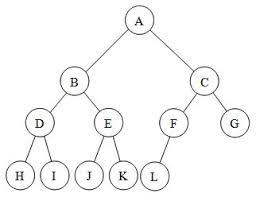
\includegraphics[width=4cm]{heap.png}
		\end{figure}
	\end{frame}

	\begin{frame}
	\frametitle{Forma alternativa}
		Arrays são uma forma cômoda de se representar esse tipo
		de árvore binária pois, utilizando a posição 1 como raiz, e
		considerando que 2*i e 2*i + 1 serão os filhos esquerdo e direito
		de 1, pode-se representar a árvore binária, sem buracos no array,
		se for completa. É possível acessar o pai também simplesmente
		dividindo a posição por 2. Esse tipo de representação está
		sendo comentado aqui pois na última aula serão estudadas dois
		tipos de árvores binárias e elas serão representadas dessa forma.
	\end{frame}

	\begin{frame}
	\frametitle{Problemas de árvores binárias}
	\begin{itemize}
	\item \textcolor{blue}{\underline{\href{https://www.urionlinejudge.com.br/judge/pt/problems/view/1195}{Árvore Binária de Busca}}}
	\item \textcolor{blue}{\underline{\href{https://www.urionlinejudge.com.br/judge/pt/problems/view/1200}{Operações em ABP I}}}
	\item \textcolor{blue}{\underline{\href{https://www.urionlinejudge.com.br/judge/pt/problems/view/1201}{Operações em ABP II}}}
	\item \textcolor{blue}{\underline{\href{https://www.urionlinejudge.com.br/judge/pt/problems/view/1191}{Recuperação da Árvore}}}
	\item \textcolor{blue}{\underline{\href{https://www.urionlinejudge.com.br/judge/pt/problems/view/1466}{Percurso em Árvore por Nível}}}
	\end{itemize}
	\end{frame}


\end{document}
